% !BIB program = biber 
\documentclass{article}

%% Encoding
\usepackage[T1]{fontenc}
\usepackage[utf8]{inputenc}

%% Fonts
% Math fonts (fourier) with utopia (erewhon) text fonts
\usepackage{fourier, erewhon}
\usepackage{algorithm}
\usepackage[noend]{algpseudocode}

%% Setup
% This package contains logos
\usepackage[autoload]{adn}
\setlogos[
\textbf{MO433 --- Intro. to Unsupervised Machine Learning}\\%[5pt]
\uppercase{Instituto de Computação --- UNICAMP}\\%[-7pt]
]%
{IC3D}%
{UNICAMP}

%% Transform section references
\makeatletter
\renewcommand*{\p@section}{\S\,}
\renewcommand*{\p@subsection}{\S\,}
\makeatother

%% Shorthands
\usepackage{xspace}
\makeatletter
\DeclareRobustCommand\onedot{\futurelet\@let@token\@onedot}
\def\@onedot{\ifx\@let@token.\else.\null\fi\xspace}

\def\eg{e.g\onedot} \def\Eg{E.g\onedot}
\def\ie{i.e\onedot} \def\Ie{I.e\onedot}
\def\cf{cf\onedot} \def\Cf{Cf\onedot}
\def\etc{etc\onedot} \def\vs{vs\onedot}
\def\wrt{w.r.t\onedot} \def\dof{d.o.f\onedot}
\def\etal{et al\onedot}
\makeatother

%%%
% Other packages start here (see the examples below)
%%

%% Figues
\usepackage{graphicx}
\graphicspath{{../output/}{./images/}}
\usepackage{caption}
\usepackage{subcaption}
\usepackage{array}
\usepackage{multirow}

%% References
% Use this section to embed your bibliography
% Instead of having a separate file, just place the bibtex entries here
\usepackage{filecontents}% create files
\begin{filecontents}{\jobname.bib}
  @misc{resnet,
    title={Deep Residual Learning for Image Recognition},
    author={Kaiming He and Xiangyu Zhang and Shaoqing Ren and Jian Sun},
    year={2015},
    eprint={1512.03385},
    archivePrefix={arXiv},
    primaryClass={cs.CV}
  }
  @misc{lars,
  Author = {Yang You and Igor Gitman and Boris Ginsburg},
  Title = {Large Batch Training of Convolutional Networks},
  Year = {2017},
  Eprint = {arXiv:1708.03888},
  }
  @misc{adam,
  Author = {Diederik P. Kingma and Jimmy Ba},
  Title = {Adam: A Method for Stochastic Optimization},
  Year = {2014},
  Eprint = {arXiv:1412.6980},
  }
  @misc{simclr,
  Author = {Ting Chen and Simon Kornblith and Mohammad Norouzi and Geoffrey Hinton},
  Title = {A Simple Framework for Contrastive Learning of Visual Representations},
  Year = {2020},
  Eprint = {arXiv:2002.05709},
  }
\end{filecontents}
% Include bibliography file
\usepackage[
backend=biber, 
style=ieee, 
natbib=true,
]{biblatex}
\addbibresource{\jobname.bib}

%% Math
\usepackage{amsmath}
\newcommand\norm[1]{\left\lVert#1\right\rVert}

%% Enumerate
\usepackage{enumitem}

\begin{document}

% Put the topic of the assignment here
\title{Project 2}
% Put your name here 
\author{
Jo\~ao Victor da Silva Guerra,
Leonardo Alves de Melo,
and Marcos Felipe de Menezes Mota
\thanks{117410, 156188 and 211893. j117410@dac.unicamp.br, leonardo.alves.melo.1995@gmail.com., and marcos.mota@ic.unicamp.br}
}

\maketitle

\begin{abstract}

  In this project, we attempt to reproduce SimCLR, which is an self-supervised framework for contrastive learning of visual representations. Contrastive learning is the learning paradigm that leverage unlabeled data to teach an algorithm to distinguish between similar and dissimilar data. The composition of data transformations, the architecture composed by a base encoder and a projection head, and the contrastive loss using the nonlinear transformation of the representation to learn the parameters improves the quality of the learned representations. Following the approach of the original paper, we evaluate the effects of batch size, optimizing algorithm, similarity function and data transformations. Finally, we trained an model for 100 epochs with the best design choices from our experiments and evaluate the final model accuracy on CIFAR-10 dataset.

\end{abstract}

\section{Introduction}

The creation of a predictive algorithm to classify images is a great challenge in machine learning and computer vision areas. Labeling every image in a dataset could be an expensive and slow task, being impossible sometimes. A way to solve that is using self-supervised algorithms, which can predict a type of class even without someone explicitly tells what are the types, they basically compares each example to another to get the similarity between them, using this comparisons to learn useful representations of the data. With such representations, a simple linear classifier on top of the self-supervised framework can predict class labels with great accuracy. Self-supervised is flexible because the learned representations can be used for other machine learning tasks like semi-supervised learning and transfer learning \cite{simclr}.  

In this project we will explore and reproduce a state-of-the-art self-supervised machine learning algorithm called SimCLR \cite{simclr}, which reached great results compared with supervised algorithms. The SimCLR accomplished one of the main goals of the self-supervision community which is to achieve supervised performance using much less data. In the paper the authors reported 85.8\% top-5 accuracy in ImageNet using 100x fewer labels than AlexNet. Our implementation will be trained over CIFAR-10 dataset and the experiments will evaluate the accuracy and best design choices.

\section{Dataset}

In our experiments, we used the CIFAR-10 dataset, which consists of 60000 colour images with 32x32 RGB pixels, totalizing 3072 features. The dataset contains 10 classes (\ie airplane, automobile, bird, cat, deer, dog, frog, horse, ship and truck) with 5000 images in the training set and 1000 images in the test set per class. We show some examples of each class in Figure \ref{fig:cifar}. 

\begin{figure}
  \centering
  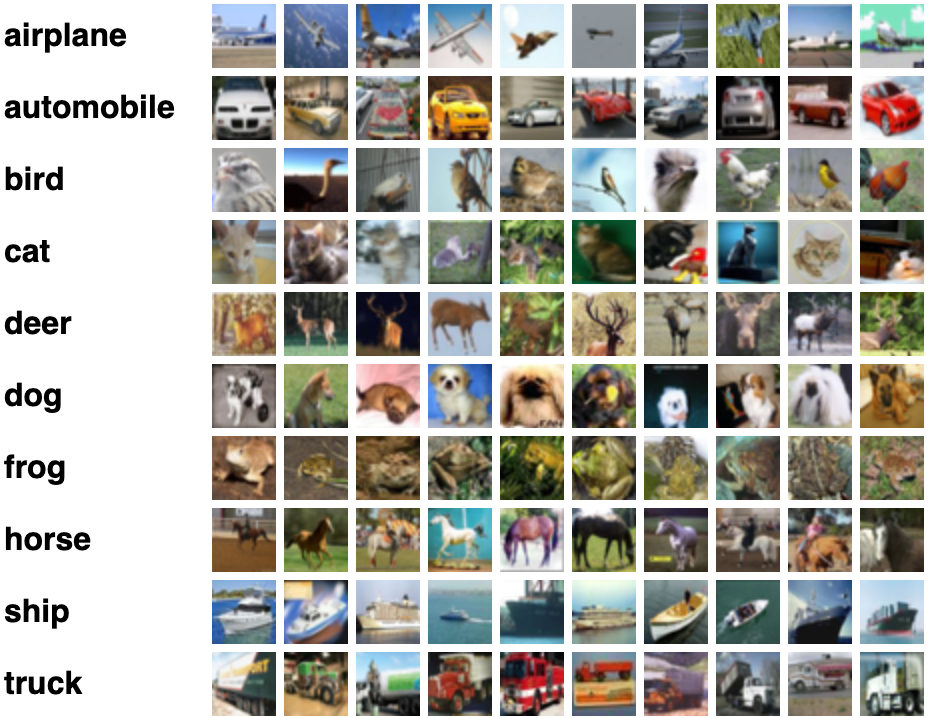
\includegraphics[width=0.8\linewidth]{cifar.png}
  \caption{Examples of CIFAR-10 classes.}
  \label{fig:cifar}
\end{figure}

\section{Implementation}

Our architecture code is divided in three main components: a data augmentation, a base encoder $f(\cdot)$ and a projection head $g(\cdot)$ modules, as can be seen in Figure \ref{fig:framework}. 

The data augmentation module randomly draws examples from the CIFAR-10 dataset, transforming each example twice using a combination of simple augmentations described in Section \ref{section:dataaug}, creating two sets ($x_i$ and $x_j$) of corresponding views. 

The base encoder $f(\cdot)$ computes the image representations ($h = f(x)$) using a convolutional neural network variant based on the ResNet architecture \cite{resnet}, which we use a resnet-50 model from \texttt{torchvision} package. The ResNet receives an augmented image $x$ of shape (32, 32, 3) and outputs a 2048-dimensional embedding vector $h$, which is our latent representation.

The projection head $g(\cdot)$ computes a non-linear projection of the image representation ($z = g(h)$) using a MultiLayer Perceptron (MLP), which has two dense layers (the first has 2048 units and the second 512 units) and the hidden layer has a non-linearity (ReLU) activation function. The MLP receives a latent representation vector $h$ of size 2048 and outputs a 128-dimensional final representation $z$. This module amplifies the invariant features and maximizes the ability of the network to identify different transformations of the same image.

\begin{figure}
  \centering
  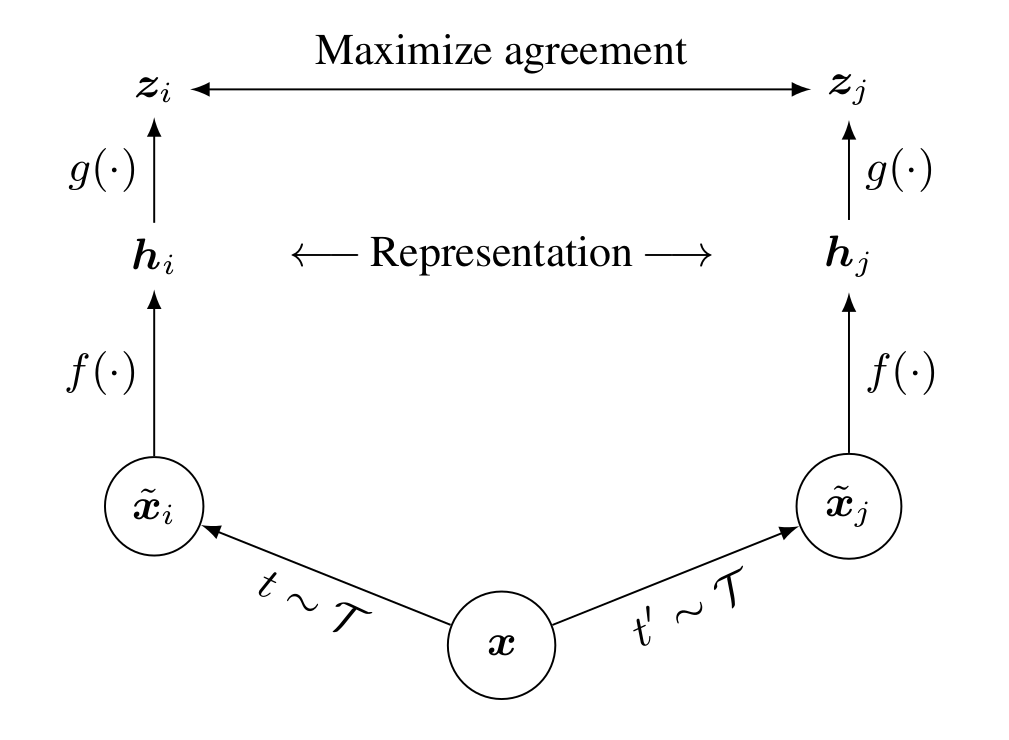
\includegraphics[width=0.7\linewidth]{framework.png}
  \caption{SimCLR Framework.}
  \label{fig:framework}
\end{figure}

\subsection{Data augmentation}
\label{section:dataaug}

Our implementation learns representations by maximizing agreement between differently augmented image of the same data example via a contrastive loss in the latent space. The data augmentation operations employed in this project include spatial/geometric transformations of data, such as cropping, resizing (with horizontal flipping) and rotation, and appearance transformation, such as color distortion and Gaussian blur. In Figure \ref{fig:exampleImage}, we show the augmentations, that we use in this project, applied to an example of our dataset.

\begin{figure}
  \begin{subfigure}[t]{0.33\textwidth}
    \centering
    \includegraphics[width=\linewidth]{images/noTransformations.png}
    \caption{Original}
  \end{subfigure}
  % \hfill
  \begin{subfigure}[t]{0.33\textwidth}
    \centering
    \includegraphics[width=\linewidth]{images/GaussianBlur.png}
    \caption{Gaussian blur}
  \end{subfigure}
  % \hfill
  \begin{subfigure}[t]{0.33\textwidth}
    \centering
    \includegraphics[width=\linewidth]{images/ColorJitter.png}
    \caption{Color distortion (jitter)}
  \end{subfigure}
  \hfill
  \begin{subfigure}[t]{0.33\textwidth}
    \centering
    \includegraphics[width=\linewidth]{images/RandomGrayScale.png}
    \caption{Color distortion (drop)}
  \end{subfigure}
  % \hfill
  \begin{subfigure}[t]{0.33\textwidth}
    \centering
    \includegraphics[width=\linewidth]{images/RandomHorizontalFlip.png}
    \caption{Horizontal flip}
  \end{subfigure}
  % \hfill
  \begin{subfigure}[t]{0.33\textwidth}
    \centering
    \includegraphics[width=\linewidth]{images/RandomResizedCrop.png}
    \caption{Crop and resize}
  \end{subfigure}
  \caption{Illustration of the data augmentation operations. Each augmentation transform data stochastically with some internal parameter.}
  \label{fig:exampleImage}
\end{figure}

\subsection{Training procedure}

The parameters of both base encoder (ResNet) and projection head (MLP) are updated through a stochastic gradient descent (SGD) to minimize the loss function of the contrastive objective.

For the similarity function, we employed a cosine similarity function ($s$; Eq. \ref{eq:cos_sim}), which measures the cosine of the angle between two non-zero d-dimensional vectors. Then, our method uses a contrastive loss function, called NT-Xent (the normalized temperature-scaled cross entropy) loss, shown in Eq. \ref{eq:ntxent}, which final value is computed across all positive pairs, $(i,j)$ and $(j,i)$, in a mini-batch.

\begin{equation}
  \label{eq:cos_sim}
  s_{i,j} = \dfrac{x_i \cdot x_j}{\norm{x_i} \cdot \norm{x_j}}
\end{equation}

\begin{equation}
  \label{eq:ntxent}
  \ell_{i,j} = -\log \dfrac{\exp (s(z_i, z_j) / \tau )}{\sum_{k=1}^{2N} \mathbb{1}_{[k \neq i]} \exp (s(z_i, z_k) / \tau )}
\end{equation}
where $\mathbb{1}_{[k \neq i]} \in {0,1}$ is an indicator function evaluating to one if and only if $k \neq i$ and $\tau$ is a temperature parameters. 

Once our system is trained, we can either directly use the output of the base encoder (ResNet) as the representation $h$ of an given image $x$, or we can use the representations $h$ to learn downstream tasks.

\section{Experiments}

First, we compared some design choices: batch size (8, 16 and 32), optimizing algorithm (Adam \cite{adam} and LARS \cite{lars}) and similarity function (cosine similarity and dot similarity). The optimizing algorithm and similarity function experiments used a batch size of 32 samples. For each of these design choices, we trained our model for 10 epochs. After, we trained our final model with the best design choices for 100 epochs.

\section{Results}

\subsection{Loss}

The NT-Xent loss function per epoch of the batch size, optimizing algorithm and similarity function experiments are shown in Figures \ref{fig:batch_loss}, \ref{fig:optim_loss} and \ref{fig:simfunc_loss}, respectively.  We observed that the loss function decreases and smoothly stabilizes in all scenarios, which is the expected behaviour for our loss function. These minimization of the loss in the latent space indicates that our models are learning representations that maximizes the agreement between our differently augmented views of the same data example.

The loss for larger batches is greater than the ones reported in the original paper. Batch size has a great impact when the number of epochs are small and stabilizes as the number of epochs used increased. The Adam optimizer showed a more stable behaviour when compared to the LARS optimizer, which was used in \cite{simclr}. Probably, the LARS would achieve a more stable behaviour if we finely tuned its parameters. Finally, the cosine similarity presented a smaller loss when compared to the dot product similarity. The difference between cosine similarity and dot product similarity is small. Thus we can see that learned representations have a normalizing factor because the angle between vectors in the representation space better define the separation of data classes.  

\begin{figure}
  \begin{subfigure}[t]{0.33\textwidth}
    \centering
    \includegraphics[width=\linewidth]{loss/batch_loss.png}
    \caption{Batch size}
    \label{fig:batch_loss}
  \end{subfigure}
  % \hfill
  \begin{subfigure}[t]{0.33\textwidth}
    \centering
    \includegraphics[width=\linewidth]{loss/optim_loss.png}
    \caption{Optimizer}
    \label{fig:optim_loss}
  \end{subfigure}
  % \hfill
  \begin{subfigure}[t]{0.33\textwidth}
    \centering
    \includegraphics[width=\linewidth]{loss/simfunc_loss.png}
    \caption{Similarity function}
    \label{fig:simfunc_loss}
  \end{subfigure}
  \caption{NT-Xent loss per epoch.}
  \label{fig:exp_loss}
\end{figure}

For our final model, we chose a batch size of 32 samples, the Adam optimizer and the cosine similarity function. The NT-Xent loss function per epoch is shown in Figure \ref{fig:final_loss}. We noted that the loss function decreases and smoothly stabilizes. However, we believe that it still does not converge completely. Hence, with more epochs and larger batch sizes, we would achieve a smaller loss and a better accuracy score.

\begin{figure}
  \begin{subfigure}[t]{0.49\textwidth}
    \centering
    \includegraphics[width=\linewidth]{loss/final_loss.png}
    \caption{NT-Xent loss per epoch}
    \label{fig:final_loss}
  \end{subfigure}
  % \hfill
  \begin{subfigure}[t]{0.49\textwidth}
    \centering
    \includegraphics[width=\linewidth]{acc/final_acc.png}
    \caption{Test accuracy per epoch}
    \label{fig:final_acc}
  \end{subfigure}
  \caption{Metrics for our final model.}
  \label{fig:final_model}
\end{figure}

\subsection{Test accuracy}

The test accuracy compare the representations of our training set with the ones of our test set, both without any augmentation. We calculate the similarity between them and evaluate if the target label for each test sample agree with the label of the most similar training sample; hence, we define the test accuracy as the number of correct labels in the test set divided by the number of test samples. 

The test accuracy per epoch of the batch size, optimizing algorithm and similarity function experiments are shown in Figures \ref{fig:batch_acc}, \ref{fig:optim_acc} and \ref{fig:simfunc_acc}, respectively. We noted that the accuracy increases in all scenarios, which is expected behaviour since our loss is decreasing. The accuracy for larger batches is greater as expected. The Adam optimizer showed a greater accuracy when compared to the LARS optimizer. Finally, the cosine similarity presented a greater accuracy loss when compared to the dot similarity.

\begin{figure}
  \begin{subfigure}[t]{0.33\textwidth}
    \centering
    \includegraphics[width=\linewidth]{acc/batch_acc.png}
    \caption{Batch size}
    \label{fig:batch_acc}
  \end{subfigure}
  % \hfill
  \begin{subfigure}[t]{0.33\textwidth}
    \centering
    \includegraphics[width=\linewidth]{acc/optim_acc.png}
    \caption{Optimizer}
    \label{fig:optim_acc}
  \end{subfigure}
  % \hfill
  \begin{subfigure}[t]{0.33\textwidth}
    \centering
    \includegraphics[width=\linewidth]{acc/simfunc_acc.png}
    \caption{Similarity function}
    \label{fig:simfunc_acc}
  \end{subfigure}
  \caption{Test accuracy per epoch.}
  \label{fig:exp_acc}
\end{figure}

For our final model, the test accuracy per epoch is shown in Figure \ref{fig:final_acc}. We observed that the accuracy increases; however, it could be higher if we trained our network with a larger batch size, more epochs and finely tuned our LARS optimizer (which achieves better results with larger batches as well).

\subsection{Data transformations}

To address the effects of different data augmentations, we trained our network for 10 epochs with different combinations of data transformations. We applied only two data transformations in the training step for each experiment and evaluated the test accuracy. The test accuracy for each combination is shown in Figure \ref{fig:transf_acc}. 

\begin{figure}
  \centering
  \includegraphics[width=0.8\linewidth]{acc/transf_acc.png}
  \caption{Top-1 test accuracy for different combination of data transformation. The diagonal corresponds to single transformations, and off-diagonals correspond to compositions of two transformations applied sequentially.}
  \label{fig:transf_acc}
\end{figure}

We realized that no single transformation was enough to learn good representations. In addition, we observed that the crop and resize operation is the most effective first transformation applied and the gaussian blur operation is the least effective. When comparing data augmentation pairs, the combination of crop resize and color jitter showed the best results. Therefore, gathering this information, we understand that some compositions of data augmentations are capable of improving the quality of the representations. Further, if we compose more than two transformations, we would achieve even better results, as happened in our final model.

\subsection{Linear Evaluation Protocol}

We also tested our final model using a process called Linear Evaluation Protocol, which consists in using the output of the encoder to train a linear classifier using the image labels as output, evaluating the quality of the representations learned by SimCLR. We used a multi-class Logistic Regression algorithm, and the accuracy of the model over the data is used to measure the feature quality.

For this project, we created encoded representations of each image in dataset, and matched to its respective labels in dataset. The group of all combinations of representation and labels was separated in 75\% for training the Logistic Regression and 25\% for testing. We got the value of 77.19\% of accuracy in training and 77.18\% in test, showing that our SimCLR has a good feature quality, considering that we trained for 10\% of the number of epochs of the original paper and the accuracy value of the paper is 90,6\%. 

\section{Conclusion}

% Check information
The attempt to reproduce a state-of-the-art framework for contrastive learning of visual representations was an important step in our learning process in the field of unsupervised machine learning. The combination of data transformations used to produce the corresponding views are critical, which prevent trivial forms of agreement. The MLP-based non-linear projection helps to identify the invariant features of each input image and improves the representation quality. Processing more examples in the same batch lead to better performance. Hence, the improvement achieved by SimCLR framework over previous methods is not due to any single design choice, but to the combination of them. Our final model with the best design choices explored achieved an Top-1 accuracy in test of 74\%. Finally, our reproduction of the SimCLR framework and showed that it is a strong and simple framework for doing further research in this direction and improve the state of self-supervised learning.


\printbibliography

\end{document}